\subsection{Recurrent Neural Networks}
\label{sub:RNN}

% Introduction
In the field of \gls{nn}, a significant breakthrough emerged with the introduction of the \gls{rnn}.\
Unlike traditional feedforward \glspl{nn}, \glspl{rnn} possess the unique capability to capture dependencies among sequential inputs.\
This section explores the evolution of the \gls{rnn} and its core constituents.
\newline
\newline
The inception of the modern \gls{rnn} is credited to the contributions of several remarkable researchers.\
Among them, Wilhelm Lenz and Ernst Isings introduced the Ising model, while John Hopfield expanded upon this concept by developing the Hopfield network, drawing inspiration from Shun'ichi Amari's adaptive model of the Ising model \citep{hopfield1982neural}.\
Finally, David Rumelhart's groundbreaking work on backpropagation in 1986 further advanced the field \citep{rumelhart1986learning}.
\newline
\newline
% Building blocks
The \gls{rnn} is a type of \gls{nn} designed to process sequential data by retaining some form of memory from previous time steps.\
This feature makes it particularly well suited to tasks such as natural language processing, speech recognition and time series analysis, where current inputs depend on previous inputs.
\newline
\newline
The architecture consists of an input $x_t$, a hidden state $h_t$, a loop over the hidden state, and the output $\hat{y_t}$ at time step $t \in \mathbb{R}$, as shown in figure \ref{fig:RNN_Architecture}.\
The unfolded view illustrates that each hidden state has its own weights, biases and activation function.\
At each time step, there are two inputs to the hidden state: the output of the previous state $h_{t-1}$, and the input at that time step $x_t$.\
The former input is multiplied by a weight matrix $W^{(hh)}$ and the latter by a weight matrix $W^{(hx)}$ to produce output features $h_t$, which are multiplied by a weight matrix $W^{(s)}$ and run through an activation function $\sigma$ to produce the prediction output $\hat{y}_t$.
\newline
\newline
The equation \ref{eq:update_hidden_state} computes the hidden state output at each time step.\
The equation \ref{eq:calculating_the_output} can then be used to calculate the prediction output at each time step by feeding in the weight matrix multiplied by the hidden state output and then passing it through an activation function $f(\cdot)$.

\myequations{Computing the next hidden state}
\begin{equation}
    \centering
    h_t = \sigma \Big( W^{(hh)}h_{t-1} + W^{(hx)}x_t \Big)
    \label{eq:update_hidden_state}
\end{equation}

\myequations{Calculating the output prediction}
\begin{equation}
    \centering
    \hat{y}_t = f\Big( W^{(s)}h_{t} \Big)
    \label{eq:calculating_the_output}
\end{equation}

\begin{figure}[ht]
    \centering
    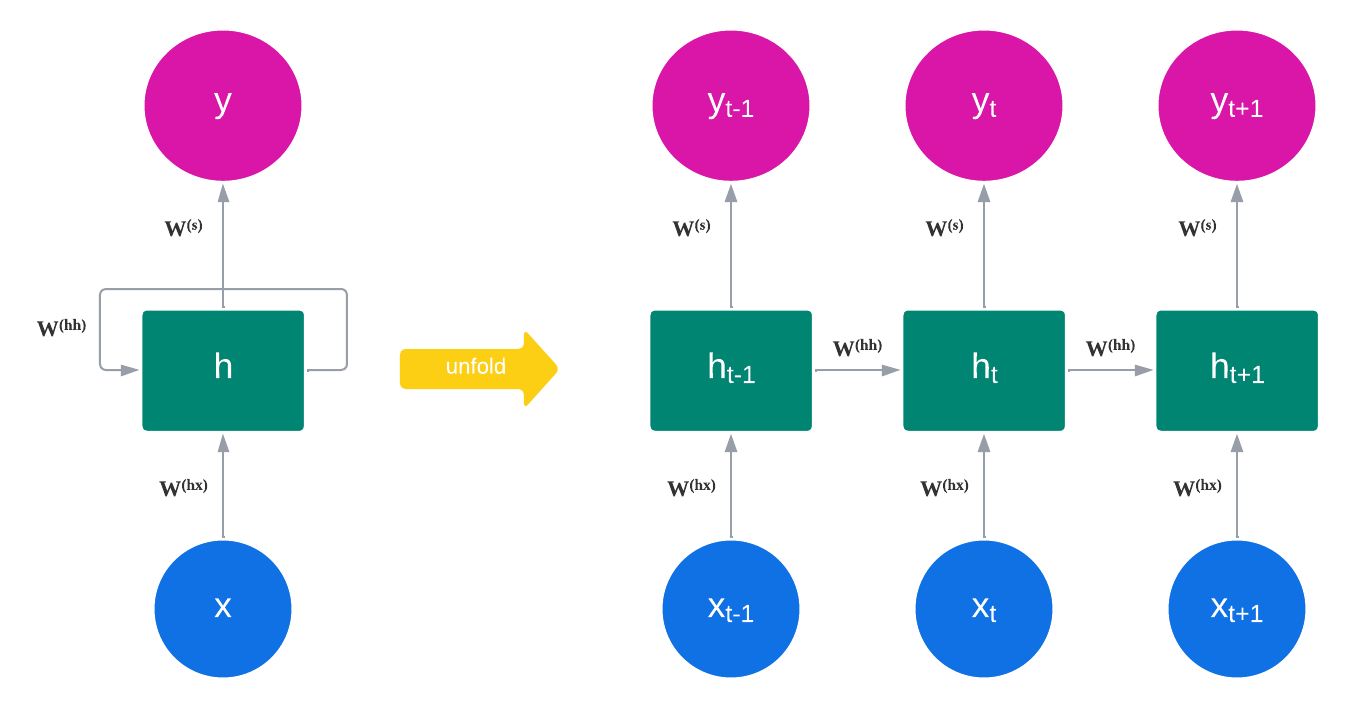
\includegraphics[width=0.75\textwidth]{./assets/img/architecture_rnn.png}
    \caption{Illustration of the folded and unfolded \gls{rnn} architecture.}
    \label{fig:RNN_Architecture}
\end{figure}

\noindent
As the same weights $W^{hh}$ and $W^{hx}$ are applied repeatedly at each time step.\
The number of parameters the model has to learn is less and, most importantly, independent of the length of the input sequence, thus defeating the curse of dimensionality.
\newline
\newline
% Training process
The training process of a \gls{rnn} is similar to that of a feedforward \gls{nn}. However, it introduces the added complexity of dealing with sequential data, where the primary objective remains the same: to minimise the calculated loss $J(\theta)$ by computing the gradients with respect to the parameters $W^{(hx)}$, $W^{(hh)}$, and $W^{(s)}$, and iteratively adjusting these parameters until they reach their optimal values.
\newline
\newline
To achieve this goal, the \gls{rnn} uses a specialised learning technique known as \gls{bptt}. Unlike traditional backpropagation used in feedforward networks, \gls{bptt} is designed to take into account the temporal nature of sequential data, making it well suited for sequential data processing. This concept was originally introduced by Werbos in 1990 \citep{werbos1990backpropagation}.
\newline
\newline
The equation \ref{eq:bptt} calculates the gradients of $J(\theta)$ with respect to $W^{(hh)}$. Since $W^{(hh)}$ is utilized in every time step up to the current output, the algorithm must backpropagate gradients from time step $t$ all the way back to initial time step $t = 0$. Once these gradients have been computed, the model parameters can be updated using equation \ref{eq:rnn_weight_update}.

\myequations{Backpropagation Through Time}
\begin{equation}
    \centering
    \frac{\partial J^{(t)}}{\partial W^{(hh)}} = \sum_{i=0}^t \frac{\partial J^{(t)}}{\partial \hat{y}^{(t)}} \cdot \frac{\partial \hat{y}^{(t)}}{\partial h_{t}} \cdot \frac{\partial h_{t}}{\partial h_{i}} \cdot \frac{\partial h_{i}}{\partial W^{(hh)}}
    \label{eq:bptt}
\end{equation}

\myequations{Updating RNN Parameters}
\begin{equation}
    \centering
    W^{(hh)} = W^{(hh)} - \alpha \cdot \frac{\partial J}{\partial W}^{(hh)}
    \label{eq:rnn_weight_update}
\end{equation}

\noindent
However, the challenge arises from the dependence of \gls{bptt} on $\frac{\partial h_t}{\partial h_i}$, which is itself a chain rule, as shown in the equation \ref{eq:unfold_chain_rule}. This leads to the vanishing gradient problem, where gradients can become progressively smaller and approach values close to zero. This happens when gradients are initially less than one and are repeatedly multiplied by gradients from earlier time steps, as shown in equation \ref{eq:vanishing_gradient_problem}. As a result, these gradients become extremely small, rendering them ineffective for parameter updates. This limitation hinders the network's ability to capture long-range dependencies in the data.

\myequations{Unfold of the chain rule for hidden state 3 to 1}
\begin{equation}
    \centering
    \frac{\partial h^{(3)}}{\partial h^{(1)}} = \frac{\partial h_{3}}{\partial h^{2}} \cdot \frac{\partial h_{2}}{\partial h^{1}}
    \label{eq:unfold_chain_rule}
\end{equation}

\myequations{Vanishing Gradient Problem}
\begin{equation}
    \centering
    \frac{\partial J^{(t)}}{\partial W^{(hh)}} = \sum_{i=0}^t \frac{\partial J^{(t)}}{\partial \hat{y}^{(t)}} \cdot \frac{\partial \hat{y}^{(t)}}{\partial h_{t}} \cdot
    \left(\prod_{j=i+1}^t \frac{\partial h_j}{\partial h_{j-1}} \right)
    \cdot
    \frac{\partial h_{i}}{\partial W^{(hh)}}
    \label{eq:vanishing_gradient_problem}
\end{equation}

\noindent
Various techniques have been developed to address the challenge of vanishing gradients, including the introduction of advanced \gls{rnn} architectures such as the \gls{lstm} network.